Le système linéaire sera de cette forme 

\begin{equation}
 x_{0} \in X^{in}, \;\;   x_{k+1}= A x_{k} ,\;\;  k \in \mathbb{N}, \;\; x_{k} \in \textbf{C}
 \end{equation}  

Où $X^{in}$ est un polytope,  
avec $A$ est une matrice donnée et $x_{k}$ représente chaque point(on suppose que c’est l’infini).\\
Le point de départ sera le triangle qui est représenté en couleur jaune et on essaye de voir la suite de trajectoire on vérifiant à chaque pas de temps ou on est.\\

\begin{figure}[ht]
	\centering
	\begin{subfigure}{.48\textwidth}
		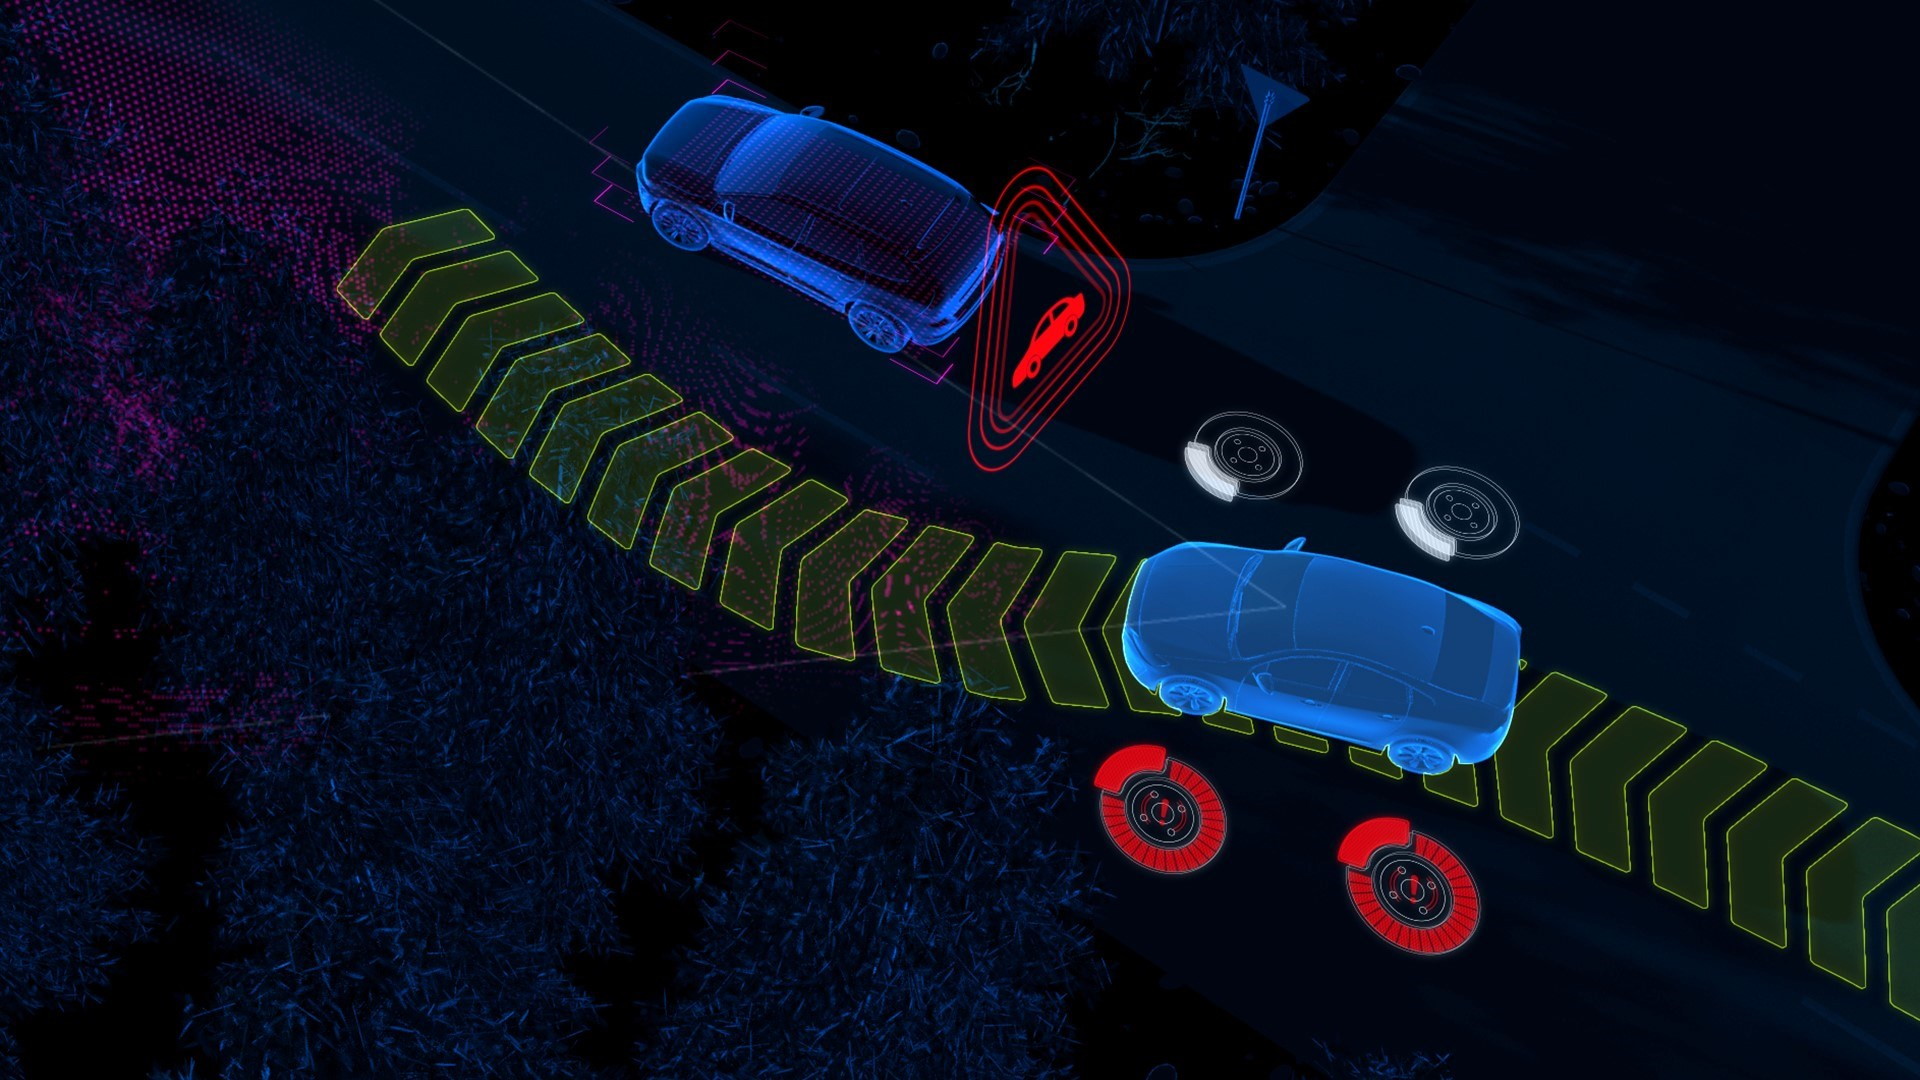
\includegraphics[width=.9\textwidth]{images/vhc1.JPG}
		\caption{}
		\label{fig:miror}
	\end{subfigure}\hfill%
	\begin{subfigure}{.48\textwidth}
		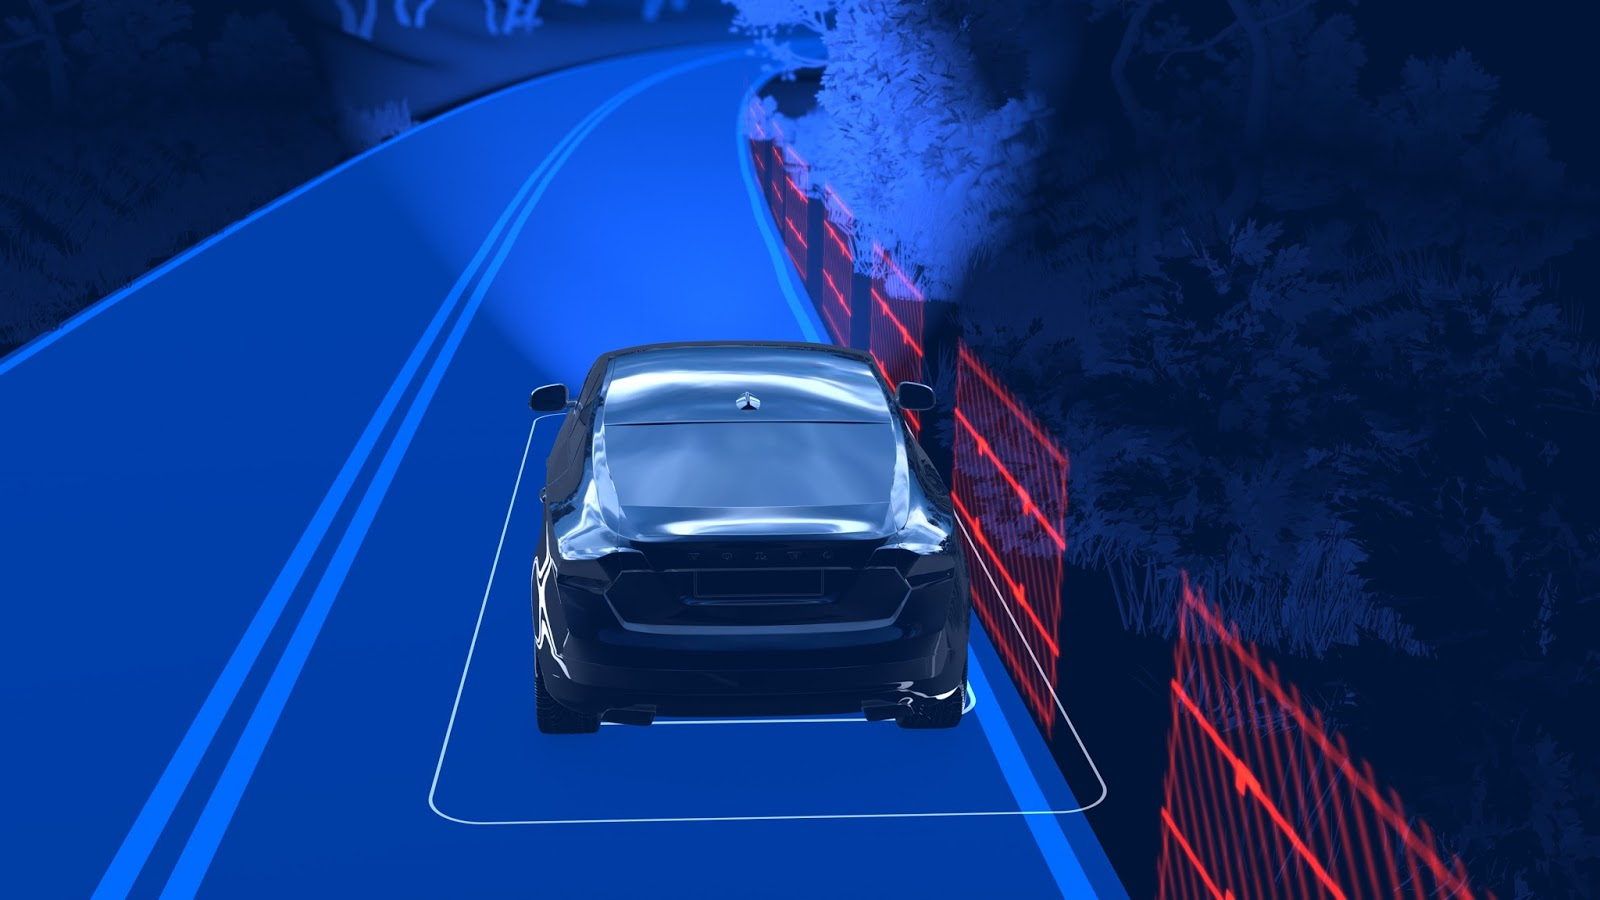
\includegraphics[width=.9\textwidth]{images/vhc2.jpg}
		\caption{}
		\label{fig:miror-couleur}
	\end{subfigure}
	\begin{subfigure}{.48\textwidth}
		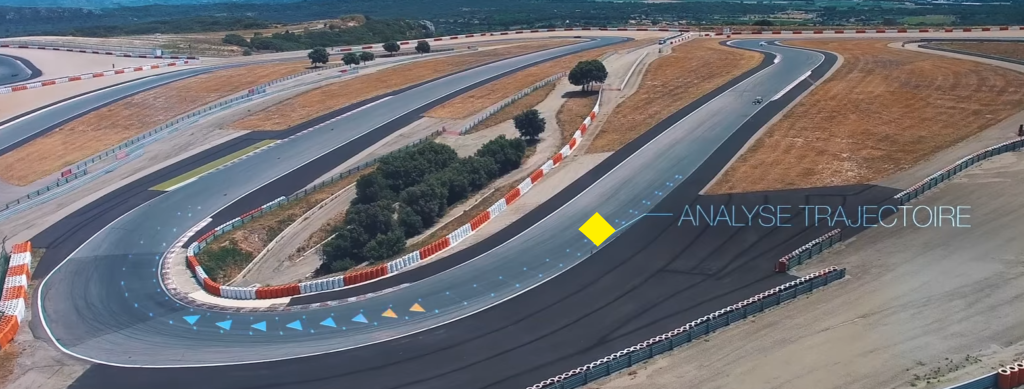
\includegraphics[width=.9\textwidth]{images/trajectoir.png}
		\caption{}
		\label{fig:miror-couleur}
	\end{subfigure}
	\caption{Analyse de trajectoire d'un véhicule autonome}
\end{figure}




 La deuxième hypothèse focalise sur l’endroit qui nous intéresse voire ou le positionnement de  véhicule dans un certain ensemble, où on peut supposé l’ensemble(la propriété) qui s’écrit sous la forme suivante:

%\edef\forall#1{\mathchar\number\forall{(#1)}\noexpand\;}

\begin{equation}
 \forall \; k \in \mathbb{N}, \;\;   x_{k} \in \{ x \in \reels^{d} / x^{T} Q x \ll \alpha  \}
 \end{equation}  
 Où $Q$ est symétrique définie positive et $\alpha \in \reels\cup \{+ \infty\}$ \\

alors l’équation 
$x^{T} Q x = ax^{2}+2bxy + cy^{2} =1$  représente une ellipse dont les axes pointent dans la direction des vecteurs propres et dont les longueurs sont $1 / \sqrt[]{\lambda_{1}},  1/ \sqrt[]{\lambda_{2}}$.
\textbf{Note}: Pour calculer une ellipse, on doit calculer le grand axe, le petit axe ça correspond au valeur propre de $Q$.


\subParagraphe{Le problème posé}
L’idée c’est de montrer finalement pour tout $x$, pour tout $k$:
\begin{itemize}
    \itemperso{} A-t-on un aperçu sur le nombre de points qui sont demandés? Le véhicule autonome va t-il s’arrêter?.
    \itemperso{} Pour faire la vérification sur le dépassement de capacité, a-t-on de variables bornées(après le calcule de la borne des $x_k$)?.
\end{itemize}

Faire preuve de sûreté, aussi preuve d’évitement face à un danger dans n'importe quelles conditions, sur n'importe quelle route. 

